\zbea
\AtBeginSection[]
{
\begin{frame}<beamer>
\frametitle{Outline}
\tableofcontents[currentsection]
\end{frame}
}

\newif\ifpdf
\ifx\pdfoutput\undefined
\pdffalse
\else
\pdfoutput=1
\pdftrue
\fi
\ifpdf

%nessim
\epstopdfsetup{suffix=}
\DeclareGraphicsRule{.eps}{pdf}{.pdf}{`epstopdf #1}
\pdfcompresslevel=9
\else

\fi

\begin{document}
%\nocite{*}

\begin{frame}
\tableofcontents
\end{frame}

\section{Linear differential equations}

\begin{frame}
\frametitle{Linear differential equations: definitions 1/2}
Linear differential equations (LDE) are of the following form:
\begin{equation*}
L[y(t)] = f(t),
\end{equation*}
where $L$ is some linear operator. \\ \pause
\ \newline
The linear operator $L$ is of the following form:
\begin{equation*}
L_n(y) = \sum_{i=0}^{n} A_i(t) \frac{d^{n-i}y}{dt^{n-i}},
\end{equation*}
with given functions $A_{1:n}$.\\ \pause
\ \newline
The \textbf{order of a LDE} is the index of the highest derivative of $y$.
\end{frame}

\begin{frame}
\frametitle{Linear differential equations: definitions 2/2}
\begin{equation*}
L_n(y) = \sum_{i=0}^{n} A_i(t) \frac{d^{n-i}y}{dt^{n-i}} = f(t).
\end{equation*}
\begin{itemize}
\item $y$ is a scalar function $\rightarrow$ \textbf{ordinary differential equation} (ODE) \pause
\item $y$ is a vector function $\rightarrow$ \textbf{partial differential equation} (PDE) \\
\ \pause
\item $f = 0$ $\rightarrow$ \textbf{homogeneous equation} \\
$\rightarrow$ solutions are called \textbf{complementary functions} \\
\ \pause
\item if $A_{0:n}(t)$ are constants (ie. not functions of time), the LDE is said to have \textbf{constant coefficients}
\end{itemize}
\end{frame}

\begin{frame}
\frametitle{Example: radioactive decay 1/2}
Let $N(t)$ be the number of radioactive atoms at time $t$, then:
\begin{equation*}
\frac{dN(t)}{dt} = - k N(t),
\end{equation*}
for some constant $k>0$. \\ \pause
\ \newline
This is a first order homogeneous LDE with constant coefficients.
\end{frame}

\begin{frame}
\frametitle{Example: radioactive decay 2/2}
\begin{figure}
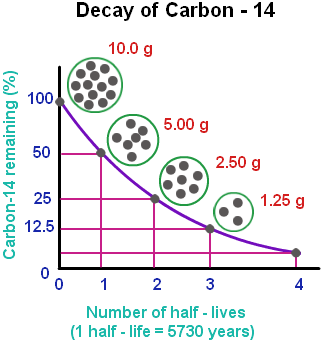
\includegraphics[width=0.5\textwidth]{decay-of-carbon-14.png}
\end{figure}
\end{frame}

\begin{frame}
\frametitle{Solving homogeneous LDEs with constant coefficients 1/3}
Solutions of LDEs must be of the form $e^{zt}$ with $z \in \mathbb{C}$. \\
\pause
\ \newline
We assume an LDE with constant coefficients:
\begin{equation*}
\sum_{i=0}^n A_i y^{(n-i)} = 0.
\end{equation*}
\ \pause
Replacing $y = e^{zt}$ leads to:
\begin{equation*}
\sum_{i=0}^n A_i z^{n-i} e^{zt} = 0
\end{equation*}
\ \pause
Dividing by $e^{zt}$ yields the $n$th order \textbf{characteristic polynomial}:
\begin{equation*}
F(z) = \sum_{i=0}^n A_i z^{n-i} = 0.
\end{equation*}
\end{frame}

\begin{frame}
\frametitle{Solving homogeneous LDEs with constant coefficients 2/3}
Characteristic equation:
\begin{equation*}
F(z) = \sum_{i=0}^n A_i z^{n-i} = 0.
\end{equation*}
\pause
\begin{enumerate}
\item Solving the polynomial $F(z)$ yields $n$ zeros $z_1$ to $z_n$.
\item Substituting a given zero $z_i$ into $e^{zt}$ gives a solution $e^{z_it}$.
\end{enumerate}
\ \newline
\pause
Homogeneous LDEs obey the superposition position: \\
$\rightarrow$ any linear combination of solutions $e^{z_1t}$,\ldots,$e^{z_nt}$ is a solution \pause \\
$\rightarrow$ $e^{z_1t}$,\ldots,$e^{z_nt}$ form a basis of the solution space of the LDE \\
\pause 
\ \newline
The specific linear combination depends on initial conditions.
\end{frame}


\begin{frame}
\frametitle{Solving homogeneous LDEs with constant coefficients 3/3}
Example:
\begin{equation*}
y^{(4)}(t) - 2 y^{(3)}(t) + 2 y^{(2)}(t) - 2 y^{(1)}(t) + y(t) = 0.
\end{equation*}
\pause
This is a 4th order homogeneous LDE with constant coefficients.\\
\ \newline
\pause
The corresponding characteristic equation:
\begin{equation*}
F(z) = z^4 - 2z^3 + 2z^2 - 2 z + 1 = 0.
\end{equation*}
\pause
The zeros of $F(z)$ are ($j=\sqrt{-1}$):
\begin{equation*}
z_1 = j, \quad z_2 = -j, \quad z_{3, 4} = 1.
\end{equation*}
\pause
These zeros correspond to the following basis functions $t$:
\begin{equation*}
 e^{jt}, \quad e^{-jt}, \quad e^t, \quad te^t.
\end{equation*}
\end{frame}

\section{Laplace transform}

\begin{frame}
\frametitle{The Laplace transform}
The Laplace transform of $f(t)$, for all real numbers $t\geq 0$:
\begin{equation*}
F(s) = \mathcal{L}\big\{f(t)\big\} = \int_0^\infty e^{-st} f(t) dt.
\end{equation*}
\pause
The parameter $s = \sigma + j\omega$ is the complex number frequency.\\ \pause
\ \newline
The initial value theorem states $f(0^+) = \lim_{s\rightarrow\infty} sF(s)$. \\
\pause
\ \newline
The final value theorem states $f(\infty) = \lim_{s\rightarrow0} sF(s)$, \\
if all poles of $sF(s)$ are in the left half plane (ie. real part $<0$).
\end{frame}

\begin{frame}
\frametitle{Important properties of the Laplace transform}
\centering
\begin{tabular}{lcc}
\textbf{property}	& \textbf{time domain}	& \textbf{$s$-domain} \\
\midrule
linearity	& $af(t)+bg(t)$ & $aF(s) + bG(s)$ \\ \pause
\ \\
differentiation	& $f^{(1)}(t)$	& $s F(s) - f(0)$ \\ \pause
\ \\
integration	& $\int_0^t f(\tau)d\tau = (u*f)(t)$	&	$\frac{1}{s}F(s)$ \\ \pause
\ \\
convolution	& $(f * g)(t)=\int_0^t f(\tau)g(t-\tau)d\tau$	& $F(s)\cdot G(s)$ \\ \pause
\ \\
time scaling	& $f(at)$	& $\frac{1}{a}F(\frac{s}{a})$ \\ \pause
\\
time shifting	& $f(t-a)u(t-a)$	& $e^{-as} F(s)$ \\ \pause
\end{tabular} \\
with $u(t)=\int_\infty^t \delta(t)dt$ (Heaviside) and $\delta(t)$ the Dirac delta.
\end{frame}


\begin{frame}
\frametitle{Inverse Laplace transform}
The inverse Laplace transform converts $s$-domain to time domain:
\begin{equation*}
f(t) = \mathcal{L}^{-1}\{F(s)\} = \frac{1}{j2\pi}\int_{\gamma-jT}^{\gamma+jT} e^{st} F(s) ds.
\end{equation*}
\pause
\ \newline
Practically, the inverse Laplace transform takes two steps:
\begin{enumerate}
\item write $F(s)$ in terms of partial fractions
\item transform each term in the partial fraction \\ based on tables of $s$/$t$-domain pairs \\ (course notes p 4.32-4.33)
\end{enumerate}
\end{frame}

\section{Solving LDEs with the Laplace transform}

\begin{frame}
\frametitle{Solving LDEs with the Laplace transform 1/3}
The Laplace transform can be used to solve LDEs with given initial conditions 
(the previous approach gave us the basis functions). \\
\pause
\ \newline
This is done by using the following property (differentiation):
\begin{align*}
\mathcal{L}\{f^{(1)}\} &= s F(s) - f(0), \\
\mathcal{L}\{f^{(2)}\} &= s^2 F(s) -s f(0) - f^{(1)}(0).
\end{align*}
\pause
Via induction, the Laplace transform of the $n$th order derivative:
\begin{equation*}
\mathcal{L}\{f^{(n)}\} = s^n F(s) - \sum_{i=1}^n s^{n-i}f^{(n-i)}(0)
\end{equation*}
\end{frame}

\begin{frame}
\frametitle{Solving LDEs with the Laplace transform 2/3}
\begin{equation*}
\mathcal{L}\{f^{(n)}\} = s^n F(s) - \sum_{i=1}^n s^{n-i}f^{(n-i)}(0)
\end{equation*}
\pause
We want to solve the following LDE:
\begin{align*}
\sum_{i=0}^{n} A_i y^{(n-i)}(t) &= f(t), \\
y^{(i)}(0) &= c_i \quad \forall i=0\ldots n.
\end{align*}
\pause
Via the linearity of the Laplace transform:
\begin{equation*}
\sum_{i=0}^{n} A_i \mathcal{L}\{y^{(n-i)}(t)\} = \mathcal{L}\{f(t)\} 
\end{equation*}
\end{frame}

\begin{frame}
\frametitle{Solving LDEs with the Laplace transform 3/3}
\begin{align}
\sum_{i=0}^{n} A_i \mathcal{L}\{y^{(n-i)}(t)\} &= \mathcal{L}\{f(t)\}  \label{firsteq} \\
\mathcal{L}\{f^{(n)}\} &= s^n F(s) - \sum_{i=1}^n s^{n-i}f^{(n-i)}(0) \label{secondeq}
\end{align}
\pause
Expanding Eq.~\eqref{secondeq} into \eqref{firsteq} yields:
\begin{equation*}
Y(s)\sum_{i=0}^n A_i s^i - \sum_{i=1}^n \sum_{j=1}^i A_i s^{i-j}y^{j-1}(0) = F(s)
\end{equation*}
\pause
The solution in the time domain is obtained via the inverse Laplace transform: $y(t) = \mathcal{L}^{-1}\{Y(s)\}$.
\end{frame}


\section{Properties of state-space representation}

\begin{frame}
\frametitle{Observability}
A measure of how well a system's internal states $\mathbf{x}$ can be inferred by knowledge of its outputs $\mathbf{y}$. \\
\pause
\ \newline
Formally, a system is said to be observable if, for any possible sequence of state and control vectors, the current state can be determined in finite time using only the outputs. \\
\ \newline
\pause
This holds for linear, time-invariant systems with $n$ states if:
\begin{equation*}
rank(\mathcal{O}) = n,\quad \mathcal{O} = \begin{bmatrix} \mathbf{C} \\ \mathbf{CA} \\ \vdots \\ \mathbf{CA}^{n-1} \end{bmatrix}, \quad \mathcal{O}: \textbf{observability matrix}
\end{equation*}

\end{frame}

\begin{frame}
\frametitle{Controllability}
A measure of the ability to move a system around in its entire configuration space using only certain admissible manipulations. \\
\ \newline
\pause
A system is controllable if its state can be moved from any initial state $\mathbf{x}_0$ to any final state $\mathbf{x}_f$ via some finite sequence of inputs $\mathbf{u}_0$\ldots$\mathbf{u}_f$. \\
\pause
\ \newline
A linear, time-invariant system with $n$ states is controllable if:
\begin{equation*}
rank(\mathcal{C}) = n,\quad \mathcal{C} = \begin{bmatrix} \mathbf{B} & \mathbf{AB} & \ldots & \mathbf{A}^{n-1}\mathbf{B} \end{bmatrix},
\end{equation*}
where $\mathcal{C}$ is called the \textbf{controllability matrix}.

\end{frame}

%%%%%%%%%%%%%%%%%%%%%%%%%%%%%%%%%%%%%%%%%%%%%%%%%%%%%%%%%%%%%%%%%%%%%%%%%%%%%%%%%%%%%%%%%%%%%%%%%%%
%%%%%%%%%%%%%%%%%%%%%%%%%%%%%%%%%%%%%%%%%%%%%%%%%%%%%%%%%%%%%%%%%%%%%%%%%%%%%%%%%%%%%%%%%%%%%%%%%%%

\section{Transfer functions}

\begin{frame}
\frametitle{Transfer function}
The transfer function of input $i$ to output $j$ is defined as:
\begin{equation*}
H_{i,j}(s) = \frac{Y_j(s)}{U_i(s)},\quad \mathbf{U}(s) = \mathcal{L}\{u(t)\},\quad \mathbf{Y}(s) = \mathcal{L}\{y(t)\}.
\end{equation*}
MIMO systems with $n$ inputs and $m$ outputs have $n\times m$ transfer functions, one for each input-output pair.\\
\ \newline
\pause
The complex Laplace variable can be rewritten: $s = \sigma + j\omega$. \\
\ \newline
\pause
The frequency response of a system can be analyzed via $\mathbf{H}(j\omega)$:
\begin{equation*}
e^{\sigma + j\omega} = e^\sigma ( \cos \omega + j \sin \omega ).
\end{equation*}
\end{frame}

\begin{frame}
\frametitle{Illustration of Euler's formula}
\begin{figure}
\centering
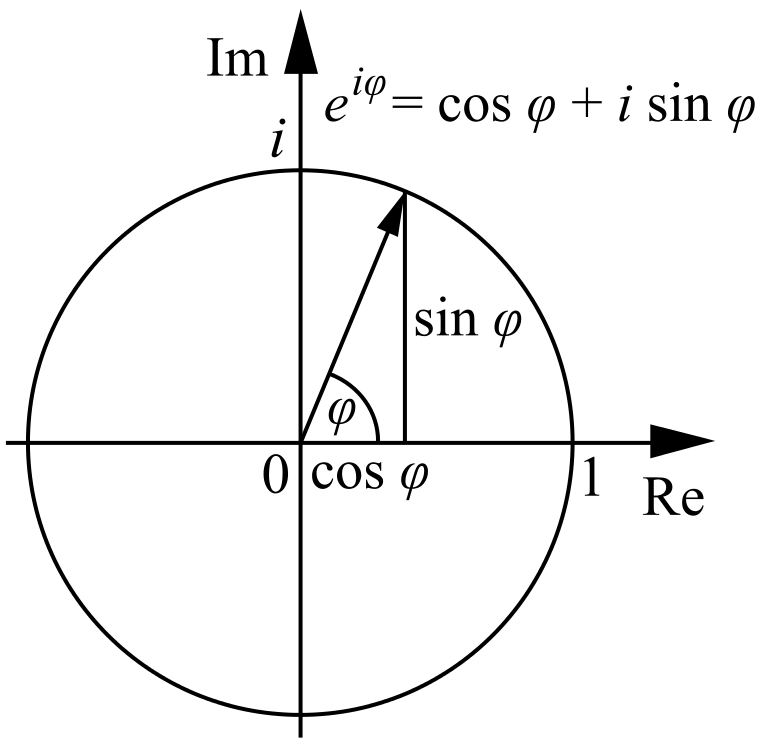
\includegraphics[width=0.5\textwidth]{euler.png}
\end{figure}
\end{frame}

\begin{frame}
\frametitle{Poles and zeros}
In general, the transfer function can be written as:
\begin{equation*}
H(s) = \frac{N(s)}{D(s)}.
\end{equation*}
\pause
The poles of $H(s)$ are zeros of $D(s)$, ie $\{s\ :\ D(s) = 0\}$.\\
\begin{itemize}
\item $|H(s)|=\infty$ if $s$ is a pole.
\end{itemize}
\ \newline
\pause
The zeros of $H(s)$ are zeros of $N(s)$, ie $\{s\ :\ N(s) = 0\}$. \\
\begin{itemize}
\item $H(s)=0$ if $s$ is a zero.
\end{itemize}
\pause
\ \newline
Poles and zeros may cancel, ie. if $D(s)=N(s)=0$ for some $s$.
\end{frame}

\begin{frame}
\frametitle{Steady state response}
The output of a linear time-invariant system yields consists of:
\begin{itemize}
\item a steady-state output $y_{ss}(t)$, which similar periodicity to $u(t)$ \\
$\rightarrow$ $y_{ss}$ comprises the same frequencies as $u(t)$ \\
\item a transient output $y_{tr}(t)$ \\
$\rightarrow$ if the system is stable, then $\lim_{t\rightarrow\infty} y_{tr}(t) = 0$  \\
$\rightarrow$ $y_{tr}(t)$ depends on the initial state $\mathbf{x}_0(t)$ of the system
\end{itemize}
\pause
\ \newline
If we apply an input $u(t) = cos(\alpha t + \theta)$, then:
\begin{equation*}
y_{ss}(t) = |H(j\alpha)|cos(\alpha t + \theta + \angle H(j\alpha))
\end{equation*}
\pause
The steady-state output $y_{ss}(t)$ of a linear time invariant system:
\begin{itemize}
\item consists of signals of same frequencies as the input signal $u(t)$
\item which may have been magnified and/or phase changed
\end{itemize}
\end{frame}

\subsection{Impulse response and time constant}

\begin{frame}
\frametitle{Impulse response}
The impulse response $h(t)$ of input $i$ to output $j$ is the output $y_j(t)$ of a system when an impulse $\delta(t)$ is applied at input $u_i(t)$.\\
\ \newline
\pause
The impulse response is the inverse Laplace transform of the transfer function $h(t) = \mathcal{L}^{-1}\{H(s)\}$.\\ 
\ \newline
\pause
For stable continuous time systems the impulse response always converges to $0$:
\begin{equation*}
\lim_{t\rightarrow\infty} h(t) = 0, \text{ because } \mathbf{D}=0 \text{ and }\lim_{t\rightarrow\infty} \mathbf{x}(t) = 0.
\end{equation*}
\pause
The speed of convergence depends on the position of the poles.
\end{frame}

\begin{frame}
\frametitle{Time constant}
The transfer function of first order systems can be written as:
\begin{equation*}
H(s) = \frac{K}{\tau s + 1}\quad \leftrightarrow \quad h(t) = \frac{K}{\tau} e^{-t/\tau},
\end{equation*}
where $\tau$ is called the system's \textbf{time constant}.\\
\ \newline
\pause
The time constant summarizes the speed of a system's dynamics:
\begin{itemize}
\item after $\tau$ seconds, the impulse response reaches $h(0)/e$.
\item after $\tau$ seconds, the step response has reached $1-e^{-1}\approx63\%$ of its regime value.
\end{itemize}
\end{frame}

\begin{frame}
\frametitle{Impulse response $H(s)=5/(5s+1) \leftrightarrow h(t)=exp(-t/5)$}
\begin{figure}
\centering
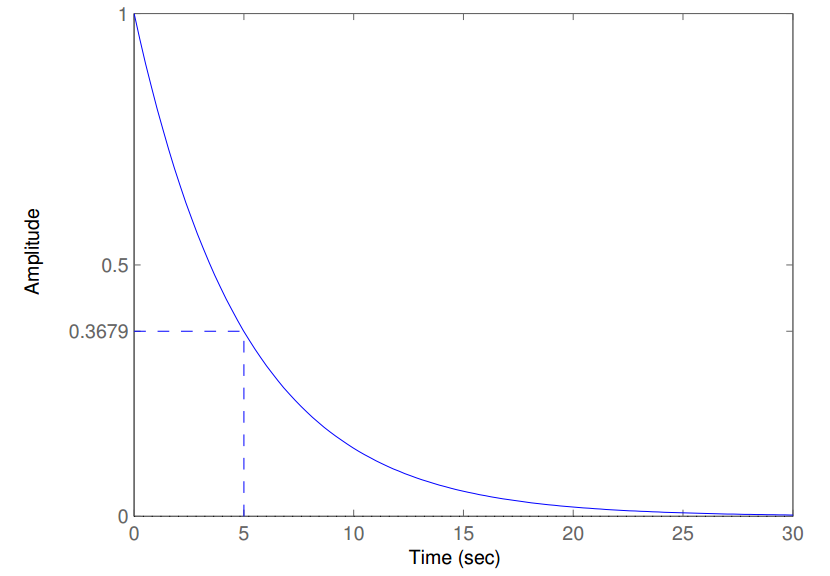
\includegraphics[width=0.8\textwidth]{time-constant-impulse.png}
\end{figure}
\end{frame}

\begin{frame}
\frametitle{Step response $H(s)=5/(5s+1) \leftrightarrow h(t)=exp(-t/5)$}
\begin{figure}
\centering
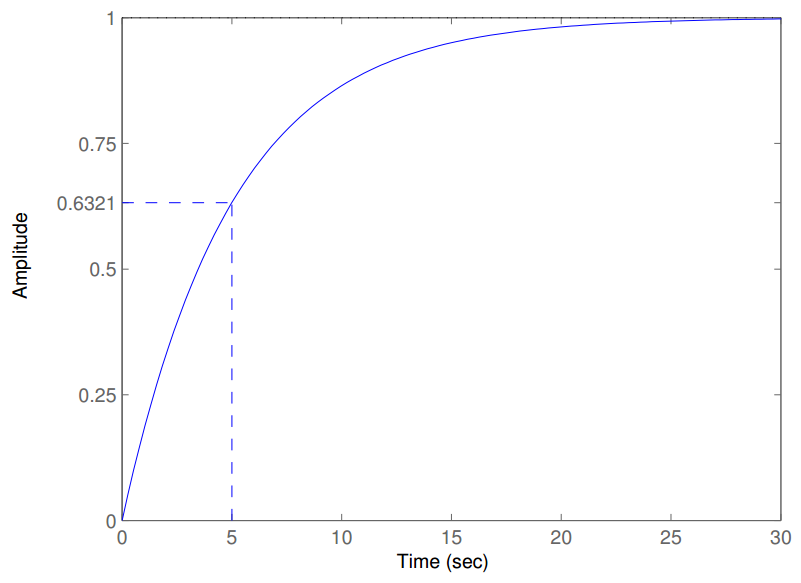
\includegraphics[width=0.8\textwidth]{time-constant-step.png}
\end{figure}
\end{frame}

\subsection{Relationship between state space and transfer functions}

\begin{frame}
\frametitle{From state-space to transfer functions}
We start from the linear state-space representation:
\begin{align*}
&\text{time domain}\hfill &\text{Laplace domain} \\
&\left\{ \begin{matrix}
\dot{\mathbf{x}}(t) = \mathbf{A} \mathbf{x}(t) + \mathbf{B} \mathbf{u}(t) \\
\mathbf{y}(t) = \mathbf{C} \mathbf{x}(t) + \mathbf{D} \mathbf{u}(t)
\end{matrix} \right. \quad\leftrightarrow\quad
&\left\{ \begin{matrix}
s \mathbf{X}(s) = \mathbf{A} \mathbf{X}(s) + \mathbf{B} \mathbf{U}(s) \\
\mathbf{Y}(s) = \mathbf{C} \mathbf{X}(s) + \mathbf{D} \mathbf{U}(s)
\end{matrix} \right.
\end{align*}
\pause
A transfer function $\mathbf{H}(s) = \frac{\mathbf{Y}(s)}{\mathbf{U}(s)}$ relates an input and an output in the Laplace-domain $\rightarrow$ to obtain it, we must eliminate $\mathbf{X}(s)$.
\pause
\begin{align*}
(s\mathbf{I}-\mathbf{A}) \mathbf{X}(s) &= \mathbf{B} \mathbf{U}(s) \\
\mathbf{X}(s) &= (s\mathbf{I}-\mathbf{A})^{-1} \mathbf{B} \mathbf{U}(s) \\
\Rightarrow \mathbf{Y}(s) &= \mathbf{C} (s\mathbf{I}-\mathbf{A})^{-1} \mathbf{B} \mathbf{U}(s) + \mathbf{D} \mathbf{U}(s) \\
\Rightarrow \hfill {\color{blue}\mathbf{H}(s)} &= {\color{blue}\mathbf{C} (s\mathbf{I}-\mathbf{A})^{-1} \mathbf{B} + \mathbf{D}}
\end{align*}
\end{frame}

\begin{frame}
\frametitle{Relationship between poles and eigenvalues of $\mathbf{A}$ 1/2}
Poles are zeros of the denominator of $\mathbf{H}(s)$, e.g. those values of $s$ for which $\mathbf{H}(s)$ is singular.\\ \pause
\ \newline
The relationship between state-space representation (matrices $\mathbf{A}$, $\mathbf{B}$, $\mathbf{C}$ and $\mathbf{D}$) and transfer functions is given by
\begin{equation*}
\mathbf{H}(s) = \mathbf{C} (s\mathbf{I}-\mathbf{A})^{-1} \mathbf{B} + \mathbf{D}
\end{equation*}
\pause
$H(s)$ cannot be computed when $(s\mathbf{I}-\mathbf{A})^{-1}$ does not exist, ie.
\begin{align*}
\det(s\mathbf{I}-\mathbf{A}) = 0
\end{align*}
\pause
The determinant is zero if $s$ is an eigenvalue of $\mathbf{A}$.\\ \pause
$\rightarrow$ {\color{blue}all poles of $\mathbf{H}(s)$ are eigenvalues of $\mathbf{A}$}
\end{frame}

\begin{frame}
\frametitle{Relationship between poles and eigenvalues of $\mathbf{A}$ 2/2}
Transfer functions only capture what is relevant to describe an input-output relationship, but not all states necessarily contribute.\pause\\
$\rightarrow$ \emph{unobservable} modes of $\mathbf{A}$ are not poles in $\mathbf{H}(s)$. \\
\pause
\ \newline
Consider the following SISO system with 2 states:
\begin{align*}
\begin{bmatrix} sX_1(s) \\ sX_2(s) \end{bmatrix} &= \begin{bmatrix} \alpha & 0 \\ 0.2 & 1 \end{bmatrix} \begin{bmatrix} X_1(s) \\ X_2(s) \end{bmatrix} + \begin{bmatrix} \beta \\ 2 \end{bmatrix} U(s) \\
Y(s) &= \begin{bmatrix} 1 & 0 \end{bmatrix} \begin{bmatrix} X_1(s) \\ X_2(s) \end{bmatrix}
\end{align*}
\pause
The transfer function $H(s) = \frac{\beta}{s-\alpha}$ has only one pole ($s_1 = \alpha$). \\
$\rightarrow$ {\color{blue}not all eigenvalues of $\mathbf{A}$ are poles in transfer functions $\mathbf{H}(s)$.}
\end{frame}


\section{Transient response analysis of first order and
second order systems}

\subsection{First order systems}

\begin{frame}
\frametitle{Transient Response}
The time response of a control system may be written as:
\begin{align*}
y(t) = y_{tr}(t) + y_{ss}(t)
\end {align*}
\\Where $y_{tr}(t)$ is the transient response and $y_{ss}(t)$ is the steady state response.
Most important characteristic of dynamic system is absolute stability.
\pause
\begin{itemize}
\item System is stable when returns to equilibrium if subject to initial condition
\item System is critically stable when oscillations of the output continue forever
\item System is unstable when output diverges without bound from equilibrium if subject to initial condition
\end{itemize}
\pause
Transient response: when input of system changes, output does not change immediately but takes time to go to steady state
\end{frame}

\begin{frame}
\frametitle{First order systems}
E.g.RC circuit, thermal system, ...
\vspace{0.25cm}
\\ 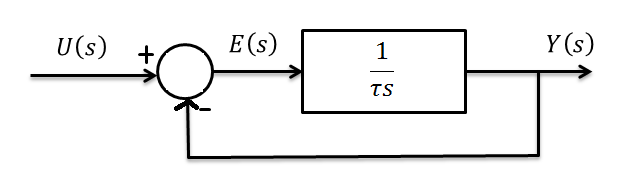
\includegraphics[width=0.7\linewidth]{Afbeelding1}
\vspace{0.5cm}
\pause
\\Transfer function is given by: $\frac{Y(s)}{U(s)} = \frac{1}{\tau s +1}$
\vspace{0.25cm}
\pause
\\Unit step response
\begin{itemize}
\vspace{0.25cm}
\item Laplace of unit-step is $\frac{1}{s}$ $\rightarrow$ substituting $U(s)= \frac{1}{s}$ \\
\vspace{0.25cm}
into equation $Y(s) = \frac{1}{s}\frac{1}{\tau s +1}$
\vspace{0.25cm}
\item Expanding into partial fractions gives
\vspace{0.25cm}
\\ $Y(s)= \frac{1}{s} - \frac{\tau}{\tau s +1} = \frac{1}{s} - \frac{1}{s+\frac{1}{\tau}}$
\end{itemize}
\end{frame}

\begin{frame}
\frametitle{Unit step transient response}
\begin{enumerate}
\item$Y(s)= \frac{1}{s} - \frac{\tau}{\tau s +1} = \frac{1}{s} - \frac{1}{s+\frac{1}{\tau}}$
\vspace{0.25cm}
\pause
\item Taking the inverse Laplace transform
\vspace{0.25cm}
\\ $y(t) = 1 - e^{-\frac{t}{\tau}}$, for $t\ge 0$ 
\vspace{0.25cm}
\pause
\item At $t=0$, the output $y(t)=0$
\vspace{0.25cm}
\pause
\item At $t=\tau$, the output $y(t)=0.632$, or $y(t)$ has reached $63.2\% $ 
\vspace{0.25cm} \\of its total change $y(\tau)= 1 - e^{-1} = 0.632$
\vspace{0.25cm}
\pause
\item Slope at time $t=0$ is $\frac{1}{\tau}$
\vspace{0.25cm}
\\ $\frac{dy}{dt}|_{t=0} = \frac{1}{\tau}e^{-\frac{t}{\tau}}|_{t=0} = \frac{1}{\tau}$
\vspace{0.25cm}
\\ Where $\tau$ is called the system time constant
\end{enumerate}
\end{frame}

\begin{frame}
\frametitle{Unit step transient response}
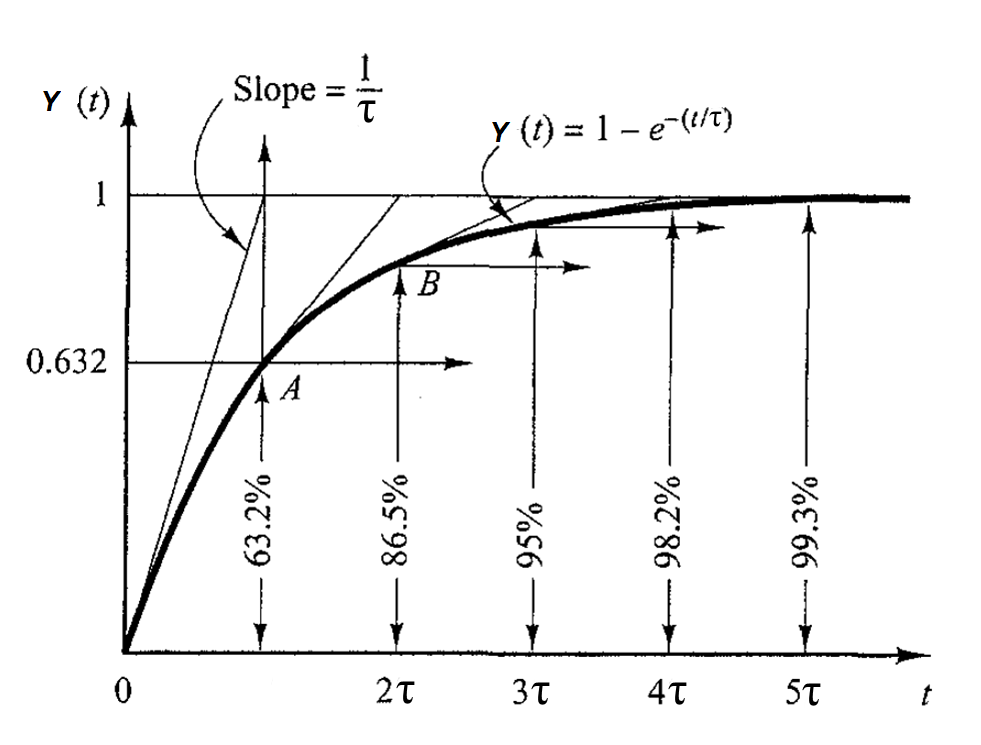
\includegraphics[width=1\linewidth]{Afbeelding2}
\end{frame}

\begin{frame}
\frametitle{Unit ramp transient response}
\begin{enumerate}
\vspace{0.25cm}
\item Laplace transform of unit ramp is $\frac{1}{s^2}$
\vspace{0.25cm}
\\ $Y(s) = \frac{1}{\tau s +1} \frac{1}{s^2}$
\vspace{0.25cm}
\pause
\item Expanding into partial fractions gives
\vspace{0.25cm}
\\ $Y(s)= \frac{1}{s^2} - \frac{\tau}{s} + \frac{\tau^2}{\tau s +1}$
\vspace{0.25cm}
\pause
\item Taking the inverse Laplace transform 
\vspace{0.25cm}
\\ $y(t) = t -\tau + \tau e^{-\frac{t}{\tau}}$, for $t\ge 0$
\vspace{0.25cm}
\pause
\item The error signal $e(t)$ is then
\vspace{0.25cm}
\\ $e(t)=u(t) -y(t) = \tau(1-e^{-\frac{t}{\tau}})$
\vspace{0.25cm}
\pause
\item For $t$ approaching infinity, $e(t)$ approaches $\tau$
\vspace{0.25cm}
\\ $e(\infty) = \tau$
\end {enumerate}
\end{frame}

\begin{frame}
\frametitle{Unit ramp transient response}
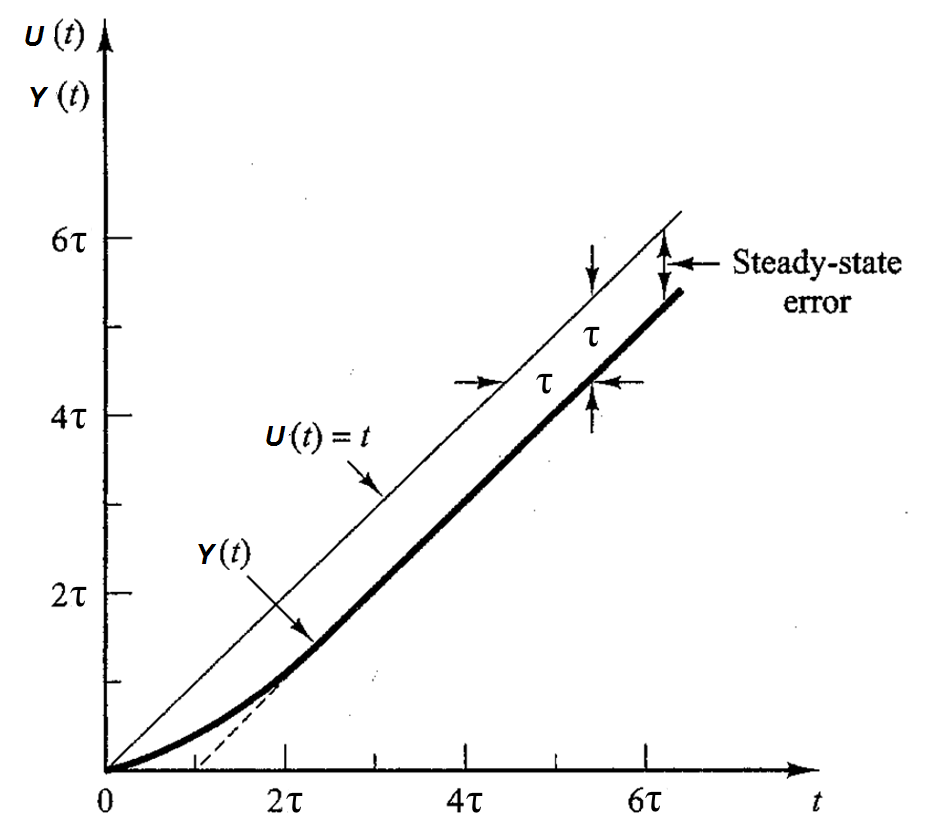
\includegraphics[width=0.8\linewidth]{Afbeelding4}
\end{frame}

\begin{frame}
\frametitle{Unit-Impulse Response}

\\ For a unit-impulse input, $U(s)=1$ and the output is
\vspace{0.2cm}
\\ 
\begin{align*}
Y(s)=\frac{1}{\tau s +1}
\end{align*}
\vspace{0.2cm}
\pause
\\ The inverse Laplace transform gives
\vspace{0.2cm}
\\
\begin{align*}
y(t)= \frac{1}{\tau}e^{-\frac{t}{\tau}} ,\text{ for } t \ge 0
\end{align*}
\vspace{0.2cm}
\pause
\\ For $t\rightarrow +\infty$, $y(t)\rightarrow 0$
\end{frame}

\begin{frame}
\frametitle{Unit-Impulse Response}
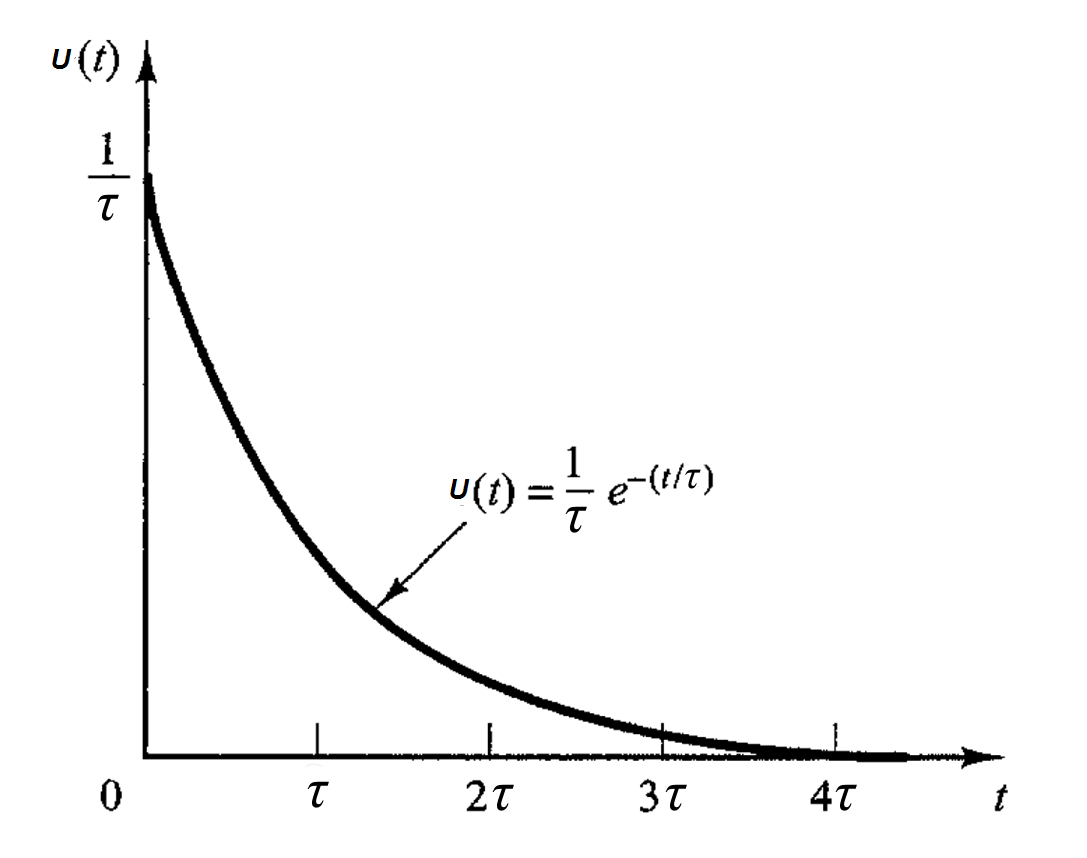
\includegraphics[width=0.8\linewidth]{Afbeelding5}
\end{frame}

\subsection{Second order systems} 

\begin{frame}
\frametitle{Second order systems}
A second order system can generally be written as:
\vspace{0.4cm}
\\ 
\begin{align*}
\frac{Y(s)}{U(s)}=H(s)=\frac{as^2+ bs+ c}{ds^2+ es+ f}
\end{align*}
\vspace{0.2cm}
\pause
\\ A system where the closed-loop transfer function possesses two poles is called a second-order system
\vspace{0.4cm}
\pause
\\ If the transfer function has two real poles, the frequency response can be found by combining the effects of both poles
\end{frame}

\begin{frame}{Second order systems} 
\vspace{-0.5cm}
\\ Sometimes the transfer function has two complex conjugate poles. In that case we have to find a different solution for finding the frequency response.
\pause
\vspace{1cm}
\\ In order to study the transient behaviour, let us first consider the following simplified example of a second order system
\\ 
\begin{align*}
H(s) = \frac{c}{ds^2+es+c}
\end {align*}
\vspace{-0.5cm}
\end{frame}

\begin{frame}
\frametitle{Step response second order system}
\begin{enumerate}
\item $H(s) = \frac{c}{ds^2+es+c}$
\vspace{0.45cm}
\pause
\item The transfer function can be rewritten as:
\\ 
\begin{align*}
H(s) &= \frac{\frac{c}{d}}{s^2+\frac{e}{d}s+\frac{c}{d}}
\\ &= \frac{\frac{c}{d}}{[s+\frac{e}{2d}+\sqrt{(\frac{e}{2d})^2-\frac{c}{d}}][s+\frac{e}{2d}-\sqrt{(\frac{e}{2d})^2-\frac{c}{d}}]}
\end{align*}
\pause
\item The poles are complex conjugates if
\\ \vspace{-0.15cm}
\begin{align*}
e^2 -4dc <0
\end{align*}
\pause
\item The poles are real if
\\
\vspace{-0.25cm}
\begin{align*}
e^2 -dc\ge 0
\end{align*}
\end{enumerate}
\end{frame}

\begin{frame}
\frametitle{Step response second order system}

\\ To simplify the transient analysis, it is convenient to write
\\ 
\begin{align*}
\frac{f}{d} = \omega_n ^2\text{, } \frac{e}{d}=2\zeta\omega_n=2\sigma
\end{align*}
\\ Where 
\\ $\sigma$ is the attenuation 
\\$\omega_n$ is the natural frequency 
\\ $\zeta$ is the damping ratio
\vspace{0.25cm}
\pause
\\ The transfer function can now be rewritten as
\\ \vspace{-0.5cm}
\begin{align*}
H(s) = \frac{\omega_n ^2}{s^2+2\zeta\omega s +\omega_n ^2}
\end{align*}
\\ Which is called the standard form of the second-order system.
\vspace{0.25cm}
\pause
\\ The dynamic behavior of the second-order system can then be described in terms of only two parameters $\zeta$ and $\omega_n$ 
\end{frame}

\begin{frame}
\frametitle{Step response second order system}
\\If $0<\zeta<1$, the poles are complex conjugates and lie in the left-half $s$-plane
\begin{itemize}
\item The system is then called \textbf{underdamped}
\vspace{0.15cm}
\item The \textbf{transient response is oscillatory}
\end{itemize}
\vspace{0.35cm}
\pause
\\ If $\zeta=0$, the \textbf{transient response doesn't die out}
\vspace{0.35cm}
\pause
\\ If $\zeta=1$, the system is called \textbf{critically damped}
\vspace{0.35cm}
\pause
\item If $\zeta>1$, the system is called \textbf{overdamped}
\vspace{0.35cm}
\\ We will now look at the unit step response for each of these cases
\end{frame}

\begin{frame}
\frametitle{Underdamped system}
\\For the underdamped case $(0< \zeta< 1)$, the transfer function can be written as:\\ 
\begin{align*}
H(s)=\frac{\omega_n ^2}{(s+\zeta\omega_n+j\omega_d)(s+\zeta\omega_n-j\omega_d)}
\end{align*}
\pause
\\Where $\omega_d$ is called the damped natural frequency
\\ 
\begin{align*}
\omega_d = \omega_n\sqrt{1-\zeta^2}
\end{align*}
\pause
\\ For a unit-step input we can write
\\ 
\begin{align*}
Y(s)=\frac{\omega_n ^2}{(s^2+2\zeta\omega_n s+\omega_n ^2)s}
\end{align*}
\end{frame}

\begin{frame}{Underdamped system}

\\ Which can be rewritten as partial fractions\\
\vspace{-0.5cm}
\begin{align*}
Y(s)&=\frac{1}{s} -\frac{s+2\zeta\omega_n}{s^2+2\zeta\omega_n s+ \omega_n ^2} \\ \vspace{2cm}
&= \frac{1}{s} -\frac{s+\zeta\omega_n}{s^2+2\zeta\omega_n s+ \omega_n ^2} -\frac{\zeta\omega_n}{s^2+2\zeta\omega_n s+ \omega_n ^2}
\end{align*}
\pause
\\ It can be shown that
\\ 
\begin{align*}
\mathcal{L}^{-1}\Big[\frac{s+\zeta\omega_n}{(s+\zeta\omega_n)^2+\omega_d ^2}\Big]&= e^{-\zeta\omega_n t}cos(\omega_d t)\\  \vspace{2cm}
\mathcal{L}^{-1}\Big[\frac{\omega_d}{(s+\zeta\omega_n)^2+\omega_d ^2}\Big]&= e^{-\zeta\omega_n t}sin(\omega_d t)
\end{align*}
\end{frame}



\begin{frame}
\frametitle{Underdamped system}
\\Therefore:\\ 
\vspace{0.25cm}
$\mathcal{L}^{-1}\Big[Y(s)\Big]=y(t)$
\vspace{0.35cm}
\pause
\\$ = 1 - e^{-\zeta\omega_n t}(cos(\omega_d t)+\frac{\zeta}{\sqrt{1 - \zeta^2}}sin(\omega_d t))$
\vspace{0.25cm}
\\$ = 1 - \frac{e^{-\zeta\omega_n t}}{\sqrt{1-\zeta^2}}sin(\omega_d t+ tan^{-1}(\frac{\sqrt{1-\zeta^2}}{\zeta}))$
\vspace{0.4cm}
\pause
\\ It can be seen that the frequency of the transient oscillation is the damped natural frequency $\omega_d$ and thus varies with the damping ratio $\zeta$
\end{frame}

\begin{frame}
\frametitle{Underdamped system}
\\ The error signal is the difference between input and output
\begin{align*}
e(t)&= y(t) -u(t)
\\&= e^{-\zeta\omega_n t}(cos(\omega_d t)+\frac{\zeta}{\sqrt{1 - \zeta^2}}sin(\omega_d t))
\end{align*}
\pause
\\ The error signal exhibits a damped sinusoidal oscillation
\vspace{0.8cm}
\pause
\\ At steady state, or at $t=\infty$, the error goes to zero
\end{frame}

\begin{frame}{Underdamped system}
\vspace{-0.5cm}
\\ If damping $\zeta=0$, the response becomes \bftext{undamped}
\pause
\begin{itemize}
\vspace{0.25cm}
\item Oscillations continue indefinitely
\vspace{0.5cm}
\pause
\item Filling in $\zeta=0$ into the equation for y(t) gives us
\\ $y(t) = 1 -cos(\omege_n t)$, for $t\ge 0$
\vspace{0.5cm}
\pause
\item We see that the system now oscillates at the natural frequency $\omega_n$
\pause
\vspace{0.5cm}
\item If a linear system has any amount of damping, the undamped natural frequency cannot be observed experimentally, only $\omega_d$ can be observed
\pause
\vspace{0.5cm}
\item $\omega_d$ is always lower than $\omega_n$
\end{itemize} 
\end{frame}

\begin{frame}
\frametitle{Critically damped system}

\\ If the two poles of the system are equal, the system is critically damped and $\zeta=1$
\vspace{0.75cm}
\pause
\\ For a unit-step, $R(s)=\frac{1}{s}$ and we can write
\begin{align*}
Y(s) =\frac{\omega_n ^2}{(s+\omega_n)^2 s}
\end{align*}
\pause
\\ The inverse Laplace transform gives us
\begin{align*}
y(t) = 1 - e^{-\omega_n t}(1+\omega_n t) \text{ for } t\ge 0
\end{align*}         
\end{frame}

\begin{frame}
\frametitle{Overdamped system}
\\ A system is overdamped ($\zeta>1$) when the two poles are negative, real and unequal
\vspace{0.5cm}
\pause
\\ For a unit-step $R(s)=\frac{1}{s}$, $Y(s)$ can be written as
\\ \vspace{-0.25cm}
\begin{align*}
Y(s) = \frac{\omega_n ^2}{(s+\zeta\omega_n + \omega_n ^2\sqrt{\zeta^2 -1})(s+\zeta\omega_n - \omega_n ^2\sqrt{\zeta^2 -1})}
\end{align*} 
\pause
\\ The inverse Laplace transform is
\\ \vspace{-0.25cm}
\begin{align*}
y(t) = 1 +\frac{w_n}{2\sqrt{\zeta^2-1}}(\frac{e^{-s_1 t}}{s1} - \frac{e^{-s_2 t}}{s2})\text{, for } t\ge 0
\end{align*}
\pause
\\ Where
\\ \vspace{-0.25cm}
\begin{align*}
s_1 = (\zeta +\sqrt{\zeta^2 -1})\omega_n\text{ and } s_2 = (\zeta -\sqrt{\zeta^2 -1})\omega_n
\end{align*}
\end{frame}

\begin{frame}
\frametitle{Overdamped system}
\\ $s_1 = (\zeta +\sqrt{\zeta^2 -1})\omega_n$ and $s_2 = (\zeta -\sqrt{\zeta^2 -1})\omega_n$
\vspace{0.3cm}
\\ Thus $y(t)$ includes two decaying exponential terms
\pause
\begin{itemize}
\vspace{0.2cm}
\pause
\item When $\zeta >> 1$, one of the two decreases much faster than the other, and then the faster decaying exponential may be neglected
\vspace{0.2cm}
\pause
\item If $-s_2$ is located much closer to the $j\omega$ axis than $-s_1$ ($|s_2|>>|s_1|$), then $-s_1$ may be neglected
\vspace{0.3cm}
\pause
\item Once the faster decaying exponential term has disappeared, the response is similar to that of a first-order system
\vspace{0.3cm}
\pause
\item In that case, $H(s)$ can be approximated by
\\ 
\begin{align*}
H(s) = \frac{\zeta\omega_n - \omega_n\sqrt{\zeta^2-1}}{s+\zeta\omega_n -\omega_n\sqrt{\zeta^2-1}}=\frac{s_2}{s+s_2}
\end{align*}
\end{itemize}
\end{frame}

\begin{frame}
\frametitle{Overdamped system}
\\ With the approximate transfer function, the unit-step response becomes
\\
\begin{align*}
 Y(s) = \frac{\zeta\omega_n - \omega_n\sqrt{\zeta^2-1}}{(s+\zeta\omega_n -\omega_n\sqrt{\zeta^2-1})s}
\end{align*}
\pause
\\ The time response for the approximate transfer function is then given as
\\ 
\begin{align*}
y(t)= 1 -e^{-(\zeta-\sqrt{\zeta^2 -1})\omega_n t}\text{, for }t\le 0
\end{align*}
\end{frame}

\begin{frame}
\frametitle{Second order systems – unit step response curves}
 Response on a step function
\\ \vspace{1cm} 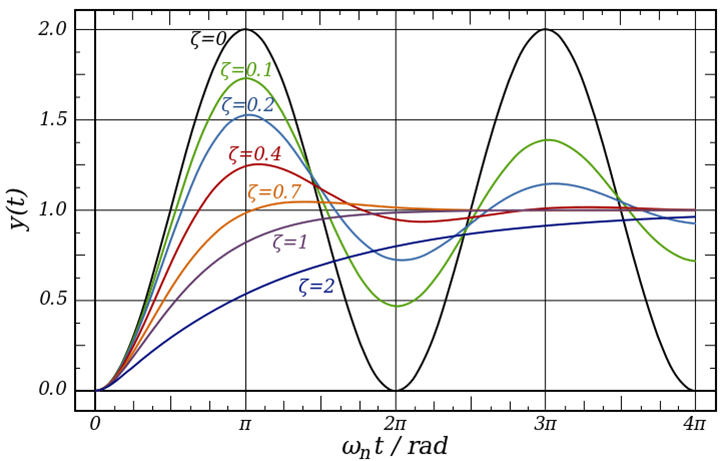
\includegraphics[width=0.8\linewidth]{Afbeelding6}
\end{frame}

\begin{frame}
\frametitle{Second order systems - characteristics}
\\ Overshoot: Highest amplitude above steady state.
\\ $M_p = e^{\frac{-\pi\zeta}{\sqrt{1-\zeta^2}}}$
\vspace{0.12cm}
\pause
\\ Rise Time: Time needed to reach the steady state for the first time. $t_r = \frac{1.8}{\omega_n}$
\vspace{0.12cm}
\pause
\\ Peak Time: Time to reach overshoot.\\$t_p =\frac{\pi}{\omega_d}$
\\ \begin{figure}
\centering{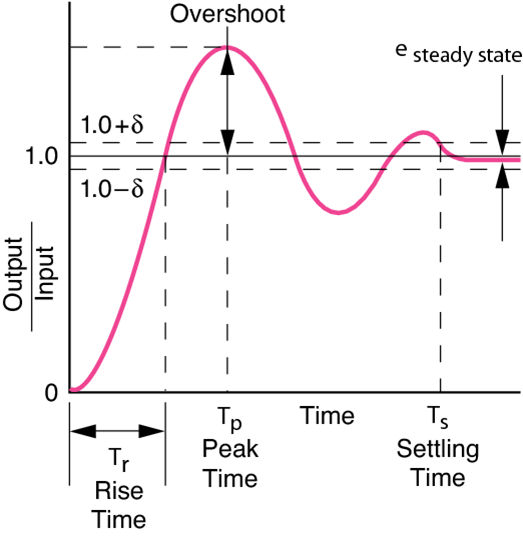
\includegraphics[width=0.4\linewidth]{Afbeelding7}}
\end{figure}
\end{frame}

\begin{frame}
\frametitle{Second order systems - characteristics}
\\ Settling Time: Time needed to approximate the steady state.
\\ $t_s = \frac{4.6}{\zeta\omega_n}$
\pause
\\ Important: this formulas are only useable for $0<\zeta<1$!
\vspace{0.15cm}
\pause
\\ For: $\delta = \frac{0.02}{\sqrt{1-\zeta^2}}$
\vspace{0.15cm}
\pause
\\ We find:
\vspace{-0.6cm}
\begin{align*}
 e^{-\zeta\omega_n T_s} &< 0.02
\\ T_s &= \frac{4}{\omega_n\zeta}
\end{align*}
\\ \begin{figure}
\centering{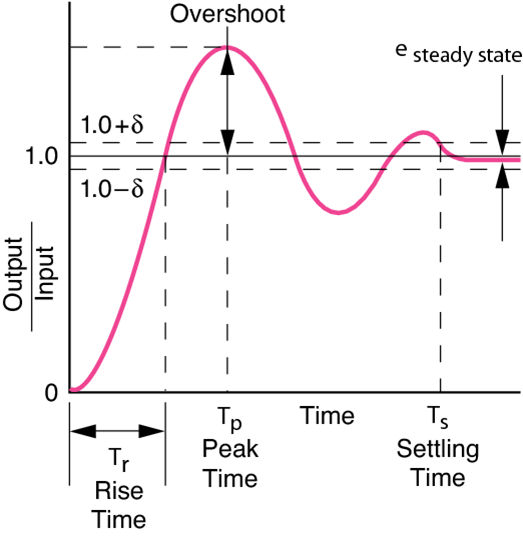
\includegraphics[width=0.35\linewidth]{Afbeelding7}}
\end{figure}
\end{frame}

\begin{frame}
\frametitle{Second order systems - resonace}
\\ The resonance frequency is the frequency at which the systems output has a larger amplitude than at other frequencies. This happens when underdamped functions oscillate at a greater magnitude than the input.
\vspace{0.35cm}
\pause
\\ An input with this frequency can sometime have catastrophic effects.
\vspace{0.35cm}
\pause
\\ A different view on the Tacoma bridge disaster: \url{https://www.youtube.com/watch?v=6ai2QFxStxo}
\vspace{0.35cm}
\\ In fact the collapse was a result of a number of effects like Aerodynamic flutter and vortices. Read the full article here: \url{http://www.ketchum.org/billah/Billah-Scanlan.pdf}
\end{frame}

\begin{frame}
\frametitle{Second order systems - resonance}
\\ The resonance frequency is: $\omega_r = \omega_n\sqrt{1-\zeta^2}$
\vspace{0.35cm}
\pause
\\ Systems with a damping $>0.707$ do not resonate
\vspace{0.35cm}
\pause
\\ The resonance frequency and the natural frequency are equal when a system has no damping.
\vspace{0.35cm}
\pause
\\ Another phenomenon with bridges and resonance is that many people marching with the same rhythm can cause a bridge to start resonating like the Angers bridge in $1850$. A more recent example is the Millennium bridge in London who started resonating.
\end{frame}

\begin{frame}
\frametitle{Second order systems - damping}

\\ When we want a system with no resonance, we choose one with damping $<0.707$. This means a pole between $135^{\circ}$ and $225^{\circ}$:
\\ 
\begin{align*}
\arctan(\frac{\sqrt{1-\zeta^2}}{\zeta}) = +135^{\circ}
\end{align*}
\pause
\\ We mostly want a short settling time ($<4$s). This results in another restriction on the poles of the system: 
\\ \begin{align*}
\tau_n= \frac{4}{\omega\zeta}&< 4\text{s}
\\ \omega_n\zeta&>1
\end{align*}
\end{frame}

\begin{frame}
\frametitle{Second order systems - damping}
\begin{figure}
\centering{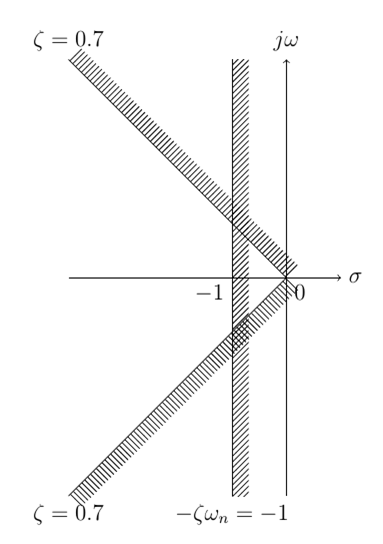
\includegraphics[width=0.5\linewidth]{Afbeelding8}}
\end{figure}
\end{frame}


